\subsection*{Pertanyaan: Analisis graf pada Gambar 8.3 dan tuliskan satu solusi jalur dengan cost minimum yang mungkin untuk kasus TSP menggunakan algoritma Branch and Bound!}

\textbf{Graf Gambar 8.3:} Edge berbobot: 0--1 = 25, 0--2 = 15, 0--3 = 20, 1--2 = 35, 1--3 = 10, dan 2--3 = 30.

\begin{figure}[H]
    \centering
    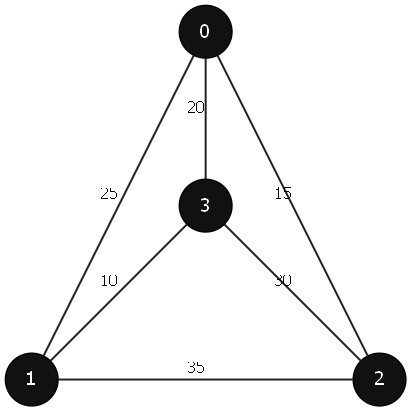
\includegraphics[width=0.48\textwidth]{figures/praktikum8/graf_pretest_83.png}
    \caption{Visualisasi Graf Pre Test dan Post Test Praktikum 8}
    \label{fig:praktikum8-graf-pretest}
\end{figure}

\textbf{Perhitungan kandidat rute:}

\begin{table}[H]
    \centering
    \caption{Perhitungan Manual Kandidat Rute TSP}
    \label{tab:praktikum8-pretest-manual}
    \begin{tabular}{ll}
    \toprule
    \textbf{Rute} & \textbf{Total Cost} \\ \midrule
    0--1--2--3--0 & 25 + 35 + 30 + 20 = 110 \\
    0--1--3--2--0 & 25 + 10 + 30 + 15 = 80 \\
    0--2--1--3--0 & 15 + 35 + 10 + 20 = 80 \\
    0--2--3--1--0 & 15 + 30 + 10 + 25 = 80 \\
    0--3--1--2--0 & 20 + 10 + 35 + 15 = 80 \\
    0--3--2--1--0 & 20 + 30 + 35 + 25 = 110 \\ \bottomrule
    \end{tabular}
\end{table}

\textbf{Jawaban:} Cost minimum adalah 80. Salah satu rute minimum:
\[
    0 \rightarrow 2 \rightarrow 1 \rightarrow 3 \rightarrow 0
\]
dengan total cost:
\[
    15 + 35 + 10 + 20 = 80
\]

\begin{figure}[H]
    \centering
    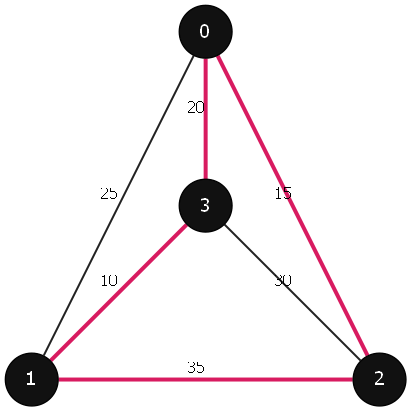
\includegraphics[width=0.48\textwidth]{figures/praktikum8/graf_pretest_83_solusi.png}
    \caption{Salah Satu Solusi Minimum TSP pada Graf Gambar 8.3}
    \label{fig:praktikum8-graf-pretest-solusi}
\end{figure}
